%! Author = zero
%! Date = 29/07/2024

\documentclass[a4paper, 12pt]{article}

\usepackage[english,russian]{babel}
\usepackage[T2A]{fontenc}
\usepackage[utf8]{inputenc}
\usepackage{geometry}
\usepackage{enumitem}
\usepackage{setspace}
\usepackage{amssymb}
\usepackage{graphicx}
\usepackage{float}
\usepackage{wrapfig}
\geometry{top=5mm}
\renewcommand{\arraystretch}{1.2}
\linespread{1}

% Document
\begin{document}
    \begin{center}
        \textbf{Задачи №1 Основы алгебры логики}
    \end{center}

    \begin{center}
        \textbf{№1 Переписать в символьном виде и посчитать:}
    \end{center}

    \begin{enumerate}
        \item $A \wedge \overline B = 1 \wedge 1 = 1$
        \item $A \vee B = 0 \vee 1 = 1$
        \item $A \vee \overline B = 0 \vee 1$
        \item $A \wedge \overline A = 0$
        \item $A \vee \overline B \vee \overline A \wedge B = (A \vee \overline B) \vee \overline{A \vee \overline B} = 1$
        \item $A \wedge B \vee C \wedge D = 1 \wedge 1 \vee 1 \wedge 1 = 1$
        \item $A \vee \overline A \wedge (B \vee C \vee D \vee E) = 1$
        \item $A \wedge B = 0 \wedge 0 = 0$

    \end{enumerate}



    \begin{center}
        \textbf{№2 Решить кругами Эйлера:}
    \end{center}

    \begin{minipage}[t]{0.4\textwidth}
        \centering
        \begin{enumerate}
            \item $A \wedge B$\\
            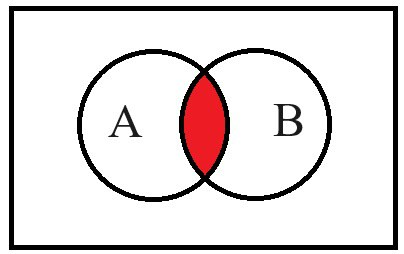
\includegraphics[width=1\linewidth]{images/im1}

            \item $\overline A \vee B$\\
            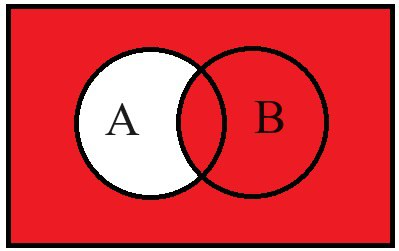
\includegraphics[width=1\linewidth]{images/im2}
        \end{enumerate}
    \end{minipage}
    \begin{minipage}[t]{0.4\textwidth}
        \centering
        \begin{enumerate}
            \setcounter{enumi}{2}
            \item $A \wedge B \wedge C$\\
            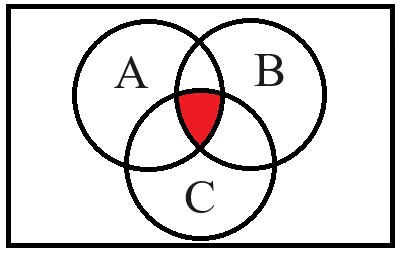
\includegraphics[width=1\linewidth]{images/im3}

            \item $A \vee \overline B$\\
            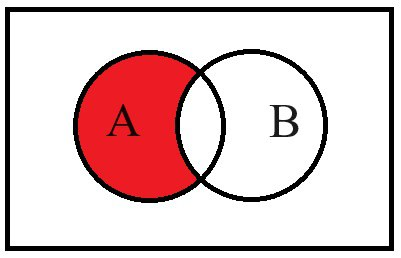
\includegraphics[width=1\linewidth]{images/im4}

        \end{enumerate}
    \end{minipage}

    \begin{center}
        \textbf{№3 Построить таблицу истинности:}
    \end{center}

    \begin{minipage}[t]{0.3\textwidth}
        \centering
        \begin{enumerate}
            \setcounter{enumi}{3}
            \begin{spacing}{1.2}
                \item $A \wedge \overline A \vee B \wedge \overline B$\\
            \end{spacing}
            \begin{tabular}{|c|c|c|}
                \hline
                $A$ & $B$ & $F$ \\
                \hline
                0   & 0   & 0   \\
                \hline
                0   & 1   & 0   \\
                \hline
                1   & 0   & 0   \\
                \hline
                1   & 1   & 0   \\
                \hline
            \end{tabular}
        \end{enumerate}
    \end{minipage}
    \begin{minipage}[t]{0.3\textwidth}
        \centering
        \begin{enumerate}
            \setcounter{enumi}{4}
            \begin{spacing}{1.2}
                \item $(A \vee \overline B) \wedge (\overline A \wedge B)$\\
            \end{spacing}
            \begin{tabular}{|c|c|c|}
                \hline
                $A$ & $B$ & $F$ \\
                \hline
                0   & 0   & 0   \\
                \hline
                0   & 1   & 0   \\
                \hline
                1   & 0   & 0   \\
                \hline
                1   & 1   & 0   \\
                \hline
            \end{tabular}
        \end{enumerate}
    \end{minipage}
    \begin{minipage}[t]{0.3\textwidth}
        \centering
        \begin{enumerate}
            \setcounter{enumi}{5}
            \begin{spacing}{1.2}
                \item $(\overline A \vee B) \wedge (A \vee \overline B)$\\
            \end{spacing}
            \begin{tabular}{|c|c|c|}
                \hline
                $A$ & $B$ & $F$ \\
                \hline
                0   & 0   & 1   \\
                \hline
                0   & 1   & 0   \\
                \hline
                1   & 0   & 0   \\
                \hline
                1   & 1   & 1   \\
                \hline
            \end{tabular}
        \end{enumerate}
    \end{minipage}


    \begin{minipage}[t]{0.22\textwidth}
        \centering
        \begin{enumerate}
            \setcounter{enumi}{0}
            \begin{spacing}{1.2}
                \item $\overline A \wedge \overline B$\\
            \end{spacing}
            \begin{tabular}{|c|c|c|}
                \hline
                $A$ & $B$ & $F$ \\
                \hline
                0   & 0   & 1   \\
                \hline
                0   & 1   & 0   \\
                \hline
                1   & 0   & 0   \\
                \hline
                1   & 1   & 0   \\
                \hline
            \end{tabular}
        \end{enumerate}
    \end{minipage}
    \begin{minipage}[t]{0.33\textwidth}
        \centering
        \begin{enumerate}
            \setcounter{enumi}{1}
            \begin{spacing}{1.2}
                \item $A \vee B \wedge \overline C$\\
            \end{spacing}
            \begin{tabular}{|c|c|c|c|}
                \hline
                $A$ & $B$ & $C$ & $F$ \\
                \hline
                0   & 0   & 0   & 0   \\
                \hline
                0   & 0   & 1   & 0   \\
                \hline
                0   & 1   & 0   & 1   \\
                \hline
                0   & 1   & 1   & 0   \\
                \hline
                1   & 0   & 0   & 1   \\
                \hline
                1   & 0   & 1   & 1   \\
                \hline
                1   & 1   & 0   & 1   \\
                \hline
                1   & 1   & 1   & 1   \\
                \hline
            \end{tabular}
        \end{enumerate}
    \end{minipage}
    \begin{minipage}[t]{0.44\textwidth}
        \centering
        \begin{enumerate}
            \setcounter{enumi}{2}
            \begin{spacing}{1.2}
                \item $A \wedge C \wedge B \wedge D$\\
            \end{spacing}
            \begin{tabular}{|c|c|c|c|c|}
                \hline
                $A$ & $B$ & $C$ & $D$ & $F$ \\
                \hline
                0   & 0   & 0   & 0   & 0   \\
                \hline
                0   & 0   & 0   & 1   & 0   \\
                \hline
                0   & 0   & 1   & 0   & 0   \\
                \hline
                0   & 0   & 1   & 1   & 0   \\
                \hline
                0   & 1   & 0   & 0   & 0   \\
                \hline
                0   & 1   & 0   & 1   & 0   \\
                \hline
                0   & 1   & 1   & 0   & 0   \\
                \hline
                0   & 1   & 1   & 1   & 0   \\
                \hline
                1   & 0   & 0   & 0   & 0   \\
                \hline
                1   & 0   & 0   & 1   & 0   \\
                \hline
                1   & 0   & 1   & 0   & 0   \\
                \hline
                1   & 0   & 1   & 1   & 0   \\
                \hline
                1   & 1   & 0   & 0   & 0   \\
                \hline
                1   & 1   & 0   & 1   & 0   \\
                \hline
                1   & 1   & 1   & 0   & 0   \\
                \hline
                1   & 1   & 1   & 1   & 1   \\
                \hline

            \end{tabular}
        \end{enumerate}
    \end{minipage}

    \begin{center}\end{center}


    \begin{center}
        \textbf{№3 Решить уравнение:}
    \end{center}

    \begin{minipage}[t]{0.3\textwidth}
        \centering
        \begin{enumerate}
            \setcounter{enumi}{0}
            \begin{spacing}{1.2}
                \item $(x \vee y) \wedge \overline x = 1$\\
            \end{spacing}
            \begin{tabular}{|c|c|c|}
                \hline
                $x$ & $y$ & $F$ \\
                \hline
                0   & 0   & 0   \\
                \hline
                0   & 1   & 1   \\
                \hline
                1   & 0   & 0   \\
                \hline
                1   & 1   & 0   \\
                \hline
            \end{tabular}
        \end{enumerate}
        Ответ: (0; 1)
    \end{minipage}
    \begin{minipage}[t]{0.4\textwidth}
        \centering
        \begin{enumerate}
            \setcounter{enumi}{1}
            \begin{spacing}{1.2}
                \item $(x \wedge y \vee x) \wedge (\overline z \wedge y \vee x) = 0$\\
            \end{spacing}
            \begin{tabular}{|c|c|c|}
                \hline
                $x$ & $y$ & $F$ \\
                \hline
                0   & 0   & 0   \\
                \hline
                0   & 1   & 0   \\
                \hline
                1   & 0   & 1   \\
                \hline
                1   & 1   & 1   \\
                \hline
            \end{tabular}
        \end{enumerate}
        Ответ: (0; 0), (0; 1)
    \end{minipage}
    \begin{minipage}[t]{0.3\textwidth}
        \centering
        \begin{enumerate}
            \setcounter{enumi}{2}
            \begin{spacing}{1.2}
                \item $\overline x \wedge y \vee x \vee y = 1$\\
            \end{spacing}
            \begin{tabular}{|c|c|c|}
                \hline
                $x$ & $y$ & $F$ \\
                \hline
                0   & 0   & 0   \\
                \hline
                0   & 1   & 1   \\
                \hline
                1   & 0   & 1   \\
                \hline
                1   & 1   & 1   \\
                \hline
            \end{tabular}
        \end{enumerate}
        Ответ: (0; 1), (1; 0), \\(1; 1)
    \end{minipage}

    \begin{center}\end{center}

    \begin{minipage}[t]{0.3\textwidth}
        \centering
        \begin{enumerate}
            \setcounter{enumi}{4}
            \begin{spacing}{1.2}
                \item $x \wedge y \vee \overline y = 0$\\
            \end{spacing}
            \begin{tabular}{|c|c|c|}
                \hline
                $x$ & $y$ & $F$ \\
                \hline
                0   & 0   & 1   \\
                \hline
                0   & 1   & 0   \\
                \hline
                1   & 0   & 1   \\
                \hline
                1   & 1   & 1   \\
                \hline
            \end{tabular}
        \end{enumerate}
        Ответ: (0; 1)
    \end{minipage}

\end{document}